	\documentclass[12pt,letterpaper]{article}

\marginparsep 0pt
\textwidth 6in
\topmargin 0pt
\headsep .5in
\textheight 8.7in
\voffset = 0pt
\hoffset = 0pt
\marginparwidth = 0pt
\oddsidemargin = 0pt

\usepackage[utf8]{inputenc}
\usepackage[spanish]{babel}
\usepackage{graphicx}
\usepackage{graphics}
\usepackage[dvips]{epsfig}
\usepackage[dvips]{graphicx}
\usepackage{rotating}
\usepackage{multirow}
\usepackage{array}
\usepackage{longtable}
\usepackage[]{fontenc}
\usepackage[nottoc,notlot,notlof]{tocbibind}


\addto\captionsspanish{
\def\listtablename{\'Indice de tablas}
\def\tablename{Tabla}
}

\begin{document}
\begin{center}
\begin{figure}[ht]
\begin{center}

\includegraphics[width=4cm]{logoUV.png}
\end{center}
\end{figure}
\thispagestyle{empty}

UNIVERSIDAD DE VALPARA\'ISO \\
Facultad de Ingenie\'ia \\
Escuela de Ingenier\'ia Civil en Inform\'atica \\
Ingenier\'ia Civil Inform\'atica\\
\vspace{1cm}
\Large
\textbf{•}\\ 
\large 
Propuesta de Trabajo de T\'itulo \\
Marcelo Esteban Verdugo Reyes \\
\normalsize
\emph{marcelo.verduor@alumnos.uv.cl} \\
\today \\
\vspace{1cm}
Profesor Gu\'ia:
Eliana Paz Providel Godoy
\end{center}



\begin{abstract}


En Chile existen diferentes familias que se encuentran en situaciones de riesgo, el cual repercute, ocasionalmente en vulneraciones de los derechos de los niños, niñas y adolescentes (NNA). Existen distintas instituciones para la protección de los integrantes de las familias dentro de estas se encuentran las corporaciones que buscan intervenir en ellas con el fin de brindar apoyo en las tareas de crianza y desarrollo personal de los NNA. 
En estas corporaciones los especialistas capacitados utilizan diferentes herramientas para analizar situaciones de riesgo en la cual se ven insertas estas familias, donde la experiencia en la toma de decisiones juega un rol fundamental. En caso de que los derechos de los NNA están siendo vulnerados, las instituciones deben actuar de inmediato. 
Estas corporaciones por lo general no disponen de herramientas Tecnologías de Informaci\'on y Comunicaci\'on (TIC) por lo cual en este Trabajo de T\'itulo se busca apoyar a los especialistas con herramientas TIC, para as\'i agilizar sus procesos y tambi\'en ser de ayuda a la hora de tomar decisiones.



\end{abstract}



\newpage

\tableofcontents
\newpage

\listoftables
\listoffigures
\newpage



\section{Introducci\'on}
\label{intr}


Uno de los derechos fundamentales de los niños, niñas y adolescentes es que sus necesidades sean satisfechas para desarrollarse y alcanzar la madurez. 
Esta tarea, principalmente recae en los padres y cuidadores, pero además de ellos, también se ven involucrados el conjunto de la sociedad en la que se encuentran los NNA. Por lo cual es necesario que cada adulto, cada comunidad y cada Estado disponga de los cuidados, la protección y la educación que estos necesitan para 

Está demostrado [Jorge Barudy, Los buenos tratos a la infancia, Primera Edición, Febrero del 2005, página 153. ] que los trastornos del desarrollo, comportamientos agresivos y violentos, así como otras manifestaciones negativas de los niños, niñas y adolescentes, tienen una estricta relación cuando estos son víctimas y testigo de violencia en el ámbito familiar.
Por lo cual es necesario prevenir los malos tratos infantiles para evitar desencadenar estas conductas negativas. 
En la región de Valparaíso existen varias poblaciones con altos porcentajes de pobreza. Una de ellas es Forestal, en donde se puede observar que los de menores de edad se caracterizan por ser víctimas de maltrato y negligencia, agresiones verbales, físicas y/o descalificaciones de mayor o menor gravedad; son testigos de violencia intrafamiliar. Entre los niños y niñas de edad preadolescente se observa bajos niveles de autoestima y percepción de logros; recurrentes problemas conductuales, malos tratos a nivel familiar y de pares, ausentismo y riesgo de deserción escolar y bajo rendimiento académico. Entre la población adolescente es posible observar conducta sexual precoz y/o de riesgo, conflictos delictuales, uso de alcohol y/o drogas, embarazo precoz, deserción escolar, microtráfico,  falta de proyectos de vida. 
Por estos motivos nacen diferentes proyectos, uno de ellos es el Programas de Prevención Focalizada PPF AITUE. El cual tiene por objetivo que los niños, niñas y adolescentes fortalezcan sus recursos personales, autoestima, autoimagen y habilidades sociales. Junto con ello, que los adultos responsables cuenten con las herramientas y oportunidades para el ejercicio de una parentalidad positiva y que las familias cuenten con apoyos para favorecer la crianza y el desarrollo de los niños, niñas y adolescentes. 
Este programa se encuentra ubicado en la población de Forestal Alto en Viña del Mar. PPF AITUE cuenta con un convenio con el Servicio Nacional de Menores (SENAME). Donde este servicio deriva a niños con riesgo social cuya residencia familiar se encuentre en la población de Forestal
PPF AITUE se encarga de utilizar acciones preventivas para influenciar positivamente las competencias parentales   y/o proporcionar recursos a las madres y los padres para que mejoren sus capacidades parentales.
 
El Programa de Prevención Focalizada PPF AITUE utiliza diferentes herramientas al momento de trabajar con las familias y los NNA.
En un principio se realiza un análisis de la situación actual de la familia. Para esto profesional se dirige al hogar de los menores para observar las condiciones en la que él y su familia conviven, además realiza entrevistas con ellos, y así con esta información obtenida,  el profesional se forma un juicio del funcionamiento familiar actual.
Posteriormente se utiliza una herramienta llamada NCFAS-G la cual ayuda al profesional a obtener una mejor apreciación de la familia.
 






\section{Definici\'on del Problema}
\label{def}

\subsection{Problema}
Actualmente los profesionales del PPF AITUE utilizan herramientas de apreciación en papel, las que posteriormente son archivadas en carpetas.
De acuerdo a lo anterior, se detecta un problema que radica en la falta de una herramienta automatizada que apoye a los profesionales del PPF AITUE la toma de decisiones. 


\subsection{Soluci\'on Propuesta}


Para dar solución a este problema se propone crear una aplicación de escritorio, la cual permitirá al profesional del PPF AITUE automatizar el proceso de apreciación familiar. Además de entregar información no trivial con respecto a procesos de apreciación anteriores realizados por otros profesionales del PPF AITUE. 

\subsection{Importancia del Trabajo}
Con este apoyo los profesionales podrían desarrollar un trabajo eficiente al momento de encontrar relaciones y patrones entre las apreciaciones de los otros profesionales (Herramienta NCFAS-G), ya sea con respecto al ingreso o bien a la salida de los NNA del PPF AITUE, con lo cual el profesional podrá:
\begin{itemize}
\item	Realizar un proceso de apreciación de manera eficiente.
\item	Realizar comparaciones con respecto a apreciaciones anteriores realizadas por otros profesionales. 
\item	Debido a las apreciaciones anteriores y a las nuevas, encontrar descriptores de la herramienta NCFAS-G que puedan alertar tempranamente problemas críticos dentro de la familia apreciada. 
\item	Entregar información con estadística descriptiva para apoyar la toma de decisiones de los profesionales.
\end{itemize}

\newpage


\begin{figure}[htb]
\begin{center}
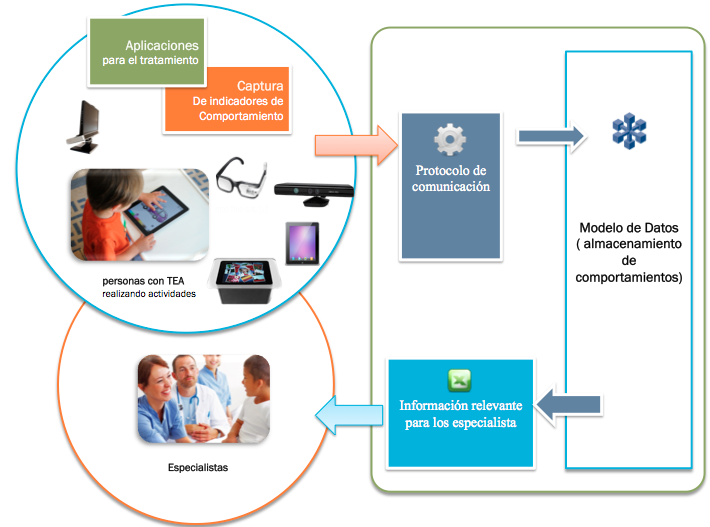
\includegraphics[width=15cm]{mono.png}
\end{center}
\caption{Dise\~no conceptual de la plataforma}
\end{figure}

En la figura 1 se describe el comportamiento de la plataforma que almacenara los 
indicadores capturados,  por un lado tenemos las aplicaciones que se utilizan para 
el tratamiento de los ni\~nos con TEA y un componente adicional que capturara los 
indicadores de comportamiento, una vez finalizada la captura de esta informaci\'on, 
ser\'a exportada a la plataforma a trav\'es de un protocolo de comunicaci\'on, quien 
realizara el nexo de la aplicaci\'on con el repositorio central, en donde ser\'an 
almacenados todos aquellos comportamientos capturados, en un an\'alisis 
posterior dichos datos almacenados podr\'an ser exportados a una planilla de
 calculo en donde podr\'an ser analizados. 

\section{Objetivos}
\label{obj}

\subsection{Objetivos generales}
El objetivo de este trabajo de título es desarrollar una aplicación que automatice la herramienta NCFAS-G utilizada en el PPF AITUE. 


\subsection{Objetivos espec\'ificos}

Para cumplir con el objetivo general es necesario cumplir los siguientes objetivos específicos:
\begin{itemize}

\item Analizar y comparar diferentes técnicas de minería de datos.
\item	Encontrar patrones dentro de los descriptores de la herramienta NCFAS-G, utilizando Minería de Datos. 
\item	Detección y predicción para la toma de decisiones basada en los datos existentes. 
\item	Implementar las técnicas de Minería de Datos seleccionada. 
\item	Generar reportes según la técnica seleccionada. 

\end{itemize}




\section{Metodolog\'ia}
\label{metod}


Para cumplir con los objetivos propuestos anteriormente, se realizará una metodología de trabajo del tipo cascada Incremental. 
Como se muestra en la Figura 1, esta metodología combina la metodología incremental la cual se lleva a cabo hasta la etapa de “Diseño”. Luego en la etapa de “Desarrollo de la primera iteración del Sistema” se da comienza a una metodología del tipo incremental, la cual perdura hasta la etapa de “Validación del Sistema” donde luego se procede a retomar la metodología incremental.
En la tabla 1 se explica cada una de las etapas que se muestran en la Figura 1.




\begin{figure}[htb]
\begin{center}
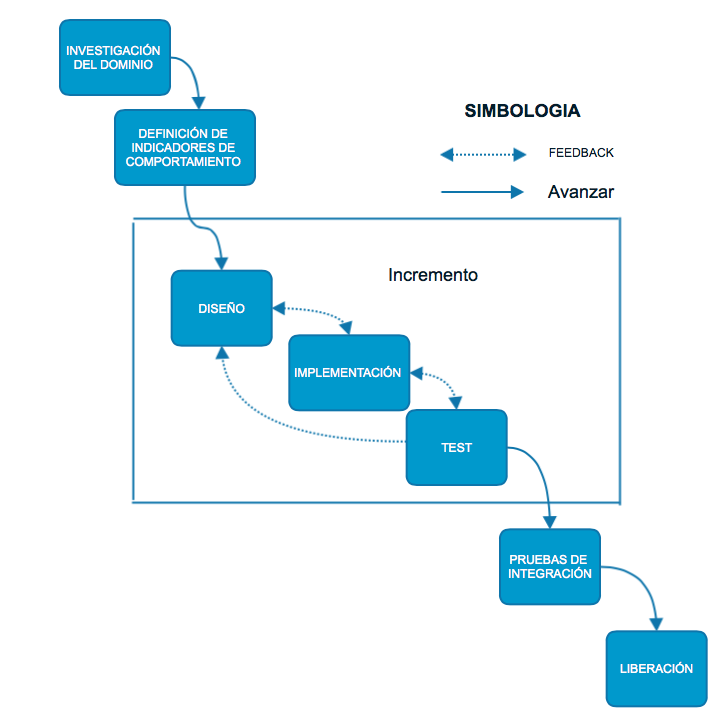
\includegraphics[width=8cm]{metodologia.png}
\end{center}
\caption{Metodolog\'ia de desarrollo del trabajo de t\'itulo}
\end{figure}



\newpage
\clearpage

\section{Planificaci\'on}
\label{plan}

Plan de desarrollo para lograr los objetivos planteados.

%% desarrollo tabla 1

\begin{table}[htf]
\begin{tabular}{| p{4cm} | c | c | p{3cm}  | p{2.5cm} |}
\hline

\multicolumn{5}{|c|}{\textbf{\textit{Planificaci\'on de Seminario de T\'itulo I 2014}}} \\ \hline \hline
\textit{\textbf{Actividades}} & 
\textit{\textbf{Inicio}} & 
\textit{\textbf{T\'ermino}} & 
\centering \textit{\textbf{Recurso}} & 
\textit{\textbf{Producto}} \\ \hline \hline
\textbf{Etapa 1: Propuesta de trabajo t\'itulo.} & 
\textbf{17/03/2014} & 
\textbf{04/04/2014} & 
\textbf{Profesor Gu\'ia, Documentos.} & 
\textbf{Propuesta Trabajo de T\'itulo} \\ \hline


Reunion 1 - Lineamiento trabajo de t\'itulo& 
18/03/2014 & 
18/03/2014 &  
Profesor gu\'ia & 
Propuesta de TT, Minuta 1.1 \\ \hline

Reunion 2 - Profesor gu\'ia & 
25/04/2014 & 
25/04/2014 &  
Profesor gu\'ia & 
Borrador 1, Minuta 1.2\\ \hline

Reunion 3 - Profesor gu\'ia & 
01/05/2014 & 
01/05/2014 &  
Profesor gu\'ia & 
Borrador 2, Minuta 1.3 \\ \hline


\hline
\end{tabular}
\caption{Planificaci\'on Etapa I}
\end{table}





%% desarrollo tabla 2

\begin{table}[htf]
\begin{tabular}{| p{4cm} | c | c | p{3cm}  | p{2.5cm} |}
\hline

\multicolumn{5}{|c|}{\textbf{\textit{Planificaci\'on de Seminario de T\'itulo I 2014}}} \\ \hline \hline
\textit{\textbf{Actividades}} & 
\textit{\textbf{Inicio}} & 
\textit{\textbf{T\'ermino}} & 
\centering \textit{\textbf{Recurso}} & 
\textit{\textbf{Producto}} \\ \hline \hline
\textbf{Etapa 2: Marco Conceptual, definici\'on del problema.} & 
\textbf{05/04/2014} & 
\textbf{25/04/2014} & 
\textbf{Profesor Gu\'ia, Libros, Internet, Expertos del dominio} & 
\textbf{Marco concept. def problema. An\'alisis de pautas e ind iniciales de comportamiento} \\ \hline


Reunion profesor gu\'ia & 
08/04/2014 & 
08/04/2014 &  
Expertos del dominio, Profesor gu\'ia & 
Borrador 1 - Minuta 2.1\\ \hline

Reunion profesor gu\'ia & 
15/04/2014 & 
15/04/2014 &  
Expertos del dominio, Profesor gu\'ia & 
Borrador 2 - Minuta 2.2 \\ \hline

Reunion profesor gu\'ia & 
22/04/2014 & 
22/04/2014 &  
Expertos del dominio, Profesor gu\'ia & 
Borrador 3 - Minuta 2.3\\ \hline


\hline
\end{tabular}
\caption{Planificaci\'on Etapa 2}
\end{table}



\newpage
\clearpage


%% desarrollo tabla 3

\begin{table}[htf]
\begin{tabular}{| p{4cm} | c | c | p{3cm}  | p{2.5cm} |}
\hline

\multicolumn{5}{|c|}{\textbf{\textit{Planificaci\'on de Seminario de T\'itulo I 2014}}} \\ \hline \hline
\textit{\textbf{Actividades}} & 
\textit{\textbf{Inicio}} & 
\textit{\textbf{T\'ermino}} & 
\centering \textit{\textbf{Recurso}} & 
\textit{\textbf{Producto}} \\ \hline \hline
\textbf{Etapa 3: Dise\~no de la soluci\'on.} & 
\textbf{26/04/2014} & 
\textbf{16/05/2014} & 
\textbf{Alumno, Profesor gu\'ia} & 
\textbf{Primera iteraci\'on de desarrollo (an\'alisis, dise\~no, implementaci\'on, modelo de datos y documentaci\'on} \\ \hline


Reunion profesor gu\'ia & 
29/04/2014 & 
29/04/2014 &  
Alumno, Profesor gu\'ia & 
An\'alisis, dise\~no ( borrador 1, Minuta 3.1)\\ \hline

Reunion profesor gu\'ia & 
06/05/2014 & 
06/05/2014 &  
Alumno, Profesor gu\'ia & 
Implementaci\'on (Borrador 2, Minuta 3.2) \\ \hline

Reunion profesor gu\'ia & 
13/05/2014 & 
13/05/2014 &  
Alumno, Profesor gu\'ia & 
Documentaci\'on (Minuta 3.3\\ \hline


\hline
\end{tabular}
\caption{Planificaci\'on Etapa 3}
\end{table}



\newpage
\clearpage

%% desarrollo tabla 4

\begin{table}[htf]
\begin{tabular}{| p{4cm} | c | c | p{3cm}  | p{2.5cm} |}
\hline

\multicolumn{5}{|c|}{\textbf{\textit{Planificaci\'on de Seminario de T\'itulo I 2014}}} \\ \hline \hline
\textit{\textbf{Actividades}} & 
\textit{\textbf{Inicio}} & 
\textit{\textbf{T\'ermino}} & 
\centering \textit{\textbf{Recurso}} & 
\textit{\textbf{Producto}} \\ \hline \hline
\textbf{Etapa 4: Implementaci\'on.} & 
\textbf{26/04/2014} & 
\textbf{16/05/2014} & 
\textbf{Alumno, Profesor gu\'ia} & 
\textbf{2da  iteraci\'on de desarrollo (an\'alisis, dise\~no implementaci\'on,) + documentaci\'on} \\ \hline


Reunion profesor gu\'ia & 
20/05/2014 & 
20/05/2014 &  
Alumno, Profesor gu\'ia & 
An\'alisis, Dise\~no, Implementaci\'on, Documentaci\'on, Minuta\\ \hline

Reunion profesor gu\'ia & 
27/05/2014 & 
27/05/2014 &  
Alumno, Profesor gu\'ia & 
An\'alisis, Dise\~no, Implementaci\'on, Documentaci\'on, Minuta\\ \hline

Reunion profesor gu\'ia & 
03/06/2014 & 
03/06/2014 &  
Alumno, Profesor gu\'ia & 
An\'alisis, Dise\~no, Implementaci\'on, Documentaci\'on, Minuta\\ \hline

Reunion profesor gu\'ia & 
10/06/2014 & 
10/06/2014 &  
Alumno, Profesor gu\'ia & 
An\'alisis, Dise\~no, Implementaci\'on, Documentaci\'on, Minuta\\ \hline

\hline
\end{tabular}

\end{table}



\newpage
\clearpage



\begin{table}[htf]
\begin{tabular}{| p{4cm} | c | c | p{3cm}  | p{2.5cm} |}
\hline

\multicolumn{5}{|c|}{\textbf{\textit{Planificaci\'on de Seminario de T\'itulo I 2014}}} \\ \hline \hline
\textit{\textbf{Actividades}} & 
\textit{\textbf{Inicio}} & 
\textit{\textbf{T\'ermino}} & 
\centering \textit{\textbf{Recurso}} & 
\textit{\textbf{Producto}} \\ \hline \hline

Reunion profesor gu\'ia & 
17/06/2014 & 
17/06/2014 &  
Alumno, Profesor gu\'ia & 
An\'alisis, Dise\~no, Implementaci\'on, Documentaci\'on, Minuta\\ \hline

Reunion profesor gu\'ia & 
24/06/2014 & 
24/06/2014 &  
Alumno, Profesor gu\'ia & 
An\'alisis, Dise\~no, Implementaci\'on, Documentaci\'on, Minuta\\ \hline

Reunion profesor gu\'ia & 
01/07/2014 & 
01/07/2014 &  
Alumno, Profesor gu\'ia & 
An\'alisis, Dise\~no, Implementaci\'on, Documentaci\'on, Minuta\\ \hline

\hline
\end{tabular}
\caption{Planificaci\'on Etapa 4}
\end{table}




\newpage
\clearpage

\section{Recursos}
\label{rec}


\subsection{Recursos Humanos}
  \begin{itemize}
    \item Profesor Gu\'ia
    \item Experto del dominio (Trastornos del Espectro Autista)
  \end{itemize}
\subsection{Hardware}
\begin{itemize}
    \item Computador: Procesador 2,3 GHz Intel Core i5, Memoria 8 GB 1333 MHz DDR3, 
    500GB de disco duro
  \end{itemize}
\subsection{Software}
  \begin{itemize}
    \item Plataforma de alta escalabilidad (hadoop).
    \item Motor de base de datos (Nosql)
    \item Netbeans (servicio rest, webservice)
  \end{itemize}

\subsection{Otros}
  \begin{itemize}
    \item Internet 
    \item Libros  
    \item Publicaciones de revistas cient\'ificas del dominio 
    (bibliotecas digitales extranjeras)  
  \end{itemize}

\newpage
\clearpage

\bibliography{propuesta}
\bibliographystyle{plain}
\end{document} 